\documentclass[a0,portrait]{a0poster}
\pagestyle{empty}
\setcounter{secnumdepth}{0}
%\usepackage{times}
\usepackage[absolute]{textpos}
\usepackage{graphics,wrapfig,times}
\usepackage{shapepar}
\usepackage{fancybox}
\usepackage{color}
\usepackage{authdate}
\usepackage[utf8x]{inputenc}
\definecolor{DarkBlue}{rgb}{0.1,0.1,0.5}
\definecolor{Red}{rgb}{0.9,0.0,0.1}
\definecolor{Black}{rgb}{0.0,0.0,0.0}
\definecolor{Green}{rgb}{0.0,0.9,0.1}

\let\Textsize\normalsize
\def\Head#1{\noindent\hbox to \hsize{\hfil{\LARGE\color{DarkBlue} #1}}\bigskip}
\def\LHead#1{\noindent{\LARGE\color{DarkBlue} #1}\smallskip}
\def\Subhead#1{\noindent{\large\color{DarkBlue} #1}}
\def\Title#1{\noindent{\Huge\color{Red} #1}}
\TPGrid[40mm,40mm]{23}{12}  % 3 - 1 - 7 - 1 - 3 Columns
%\TPGrid[25mm,20mm]{80}{114}  % 1 unit ~ 1 cm
\parindent=0pt
\parskip=0.5\baselineskip
\newcommand{\ddd}{\,\mathrm{d}}

   \setlength{\paperwidth}{87cm}
   \setlength{\paperheight}{119cm}
   \setlength{\textwidth}{87cm}
   \setlength{\textheight}{114cm}


\begin{document}

%%%%%%%%%%%%%%%%%%%%%%%%%%%%%%%%%%%%%%%%%%%%%%%%%%%%%%%%%%%%%%%%%%%%%%%%%%%%%%%%%%%%%%%%%%%%%%
                                % TITRES



\begin{textblock}{20}(1,0)
\begin{center}
\shadowbox{
\hspace{2cm}
\begin{minipage}{32cm}
%  \vspace{2cm} \baselineskip=3\baselineskip
  \Title{\begin{center}A Common GPU n-Dimensional Array for Python and C\end{center}} %\vspace{1cm}
\end{minipage}
\hspace{2cm}
}
\end{center}
\end{textblock}

\begin{textblock}{3}(18,0.1)
\doublebox{
\hspace{1.5cm}
\begin{minipage}{15cm}
\vspace{.5cm}
\LHead{Frédéric Bastien}\\
\LHead{Arnaud Bergeron}\\
\LHead{Andreas Klöckner}\\
\LHead{Pascal Vincent}\\
\LHead{Yoshua Bengio}
\end{minipage}
}
\end{textblock}


\begin{textblock}{3}(-.3,0)
\scalebox{0.8}{\includegraphics{UdeM_NoirBleu_logo_Marie_crop.pdf}}
\end{textblock}

\begin{textblock}{20}(-2,1.)
{\color{DarkBlue}{\vrule depth 0pt height 0.5cm width 125cm}}
\end{textblock}


%%%%%%%%%%%%%%%%%%%%%%%%%%%%%%%%%%%%%%%%%%%%%%%%%%%%%%%%%%%%%%%%%%%%%%%%%%
%%% Common Framework

\begin{textblock}{12}(0,1.5)
  \Ovalbox{
    \hspace{1cm}
     \begin{minipage}{35.85cm}
       \vspace{1cm}
           \begin{center}
      {\huge Why do we need this?}
    \end{center}
           \begin{itemize}
\item Efficient linear algebra is a the core of many scientific applications
\item On the CPU, numpy ndarray provides a standard object (for python at least)
\end{itemize}
           \begin{center}
      {\huge Why a new implementation?}
    \end{center}
%\begin{block}
{There are already a number of existing GPU computing codebases:}
Theano, PyCUDA/PyOpenCL, CUDAmat, Gnumpy, Thrust, ...
%\end {block}
\begin{enumerate}
\item All are incompatible
\item They do not support the full range of numpy ndarray features
\item None support both CUDA and OpenCL
\end{enumerate}
       \vspace{1cm}
     \end{minipage}
     \hspace{1cm}
   }

 \end{textblock}


%%%%%%%%%%%%%%%%%%%%%%%%%%%%%%%%%%%%%%%%%%%%%%%%%%%%%%%%%%%%%%%%%%%%%%%%%%%%%%%%%%%%%%%%%%%%%%%%%%
%%% Empirical results

\begin{textblock}{12}(0,3.2)

\Ovalbox{
{\color{Black}
\hspace{1cm}
\begin{minipage}{35.85cm}
  \vspace{1cm}

      \begin{center}
      {\huge Features desired}
   \end{center}

\begin{itemize}
\item Support for varying datatypes
\item Support for an arbitrary number of dimensions
\item Support for strides
\item Support for broadcasting
\item Compatibility with CUDA and OpenCL
\end{itemize}
\vspace{1cm}

      \begin{center}
      {\huge Easy to develop}
   \end{center}

\begin{itemize}
\item Not always a good idea to make a gpu code work for all memory layout.
  \begin{itemize}
  \item Harder to code
  \item Harder to get efficient
  \end{itemize}
\item Just call \begin{bf}as\_\{contiguous,fortran\}\_memory()\end{bf}
 on inputs!
\end{itemize}

\end{minipage}
\hspace{1cm}
}}
\end{textblock}
 
\begin{textblock}{12}(0,5.4)

\Ovalbox{
{\color{Black}
\hspace{1cm}
\begin{minipage}{35.85cm}
  \vspace{1cm}

\begin{center}
      {\huge Why has this not been done before?}
   \end{center}
\begin{itemize}
\item Hard and time consuming to get right and efficient
\item Certain algorithms cannot work on a general memory layout
\item Indexing computations take up a significant portion of time on the GPU
\end{itemize}


\end{minipage}
\hspace{1cm}
}}
\end{textblock}


\begin{textblock}{12}(0,6.2)

\Ovalbox{
{\color{Black}
\hspace{1cm}
\begin{minipage}{35.85cm}
  \vspace{1cm}

      \begin{center}
      {\huge Strides}
   \end{center}

\begin{itemize}
\item Strides is a way to specify how much memory to skip between each element of a dimension.
\item We can use strides to take submatrix B without copying any memory.
%%\only<2>{We can use strides to take submatrix ${\color{cyan!50}B}$ without copying any memory.}
\item Matrix A\hspace{5em}Matrix B
%%\onslide<1->{Matrix ${\color{red!50}A}$}\hspace{5em}\onslide<2->{Matrix ${\color{cyan!50}B}$}
\end{itemize}
\begin{center}
\end{center}
\begin{center}
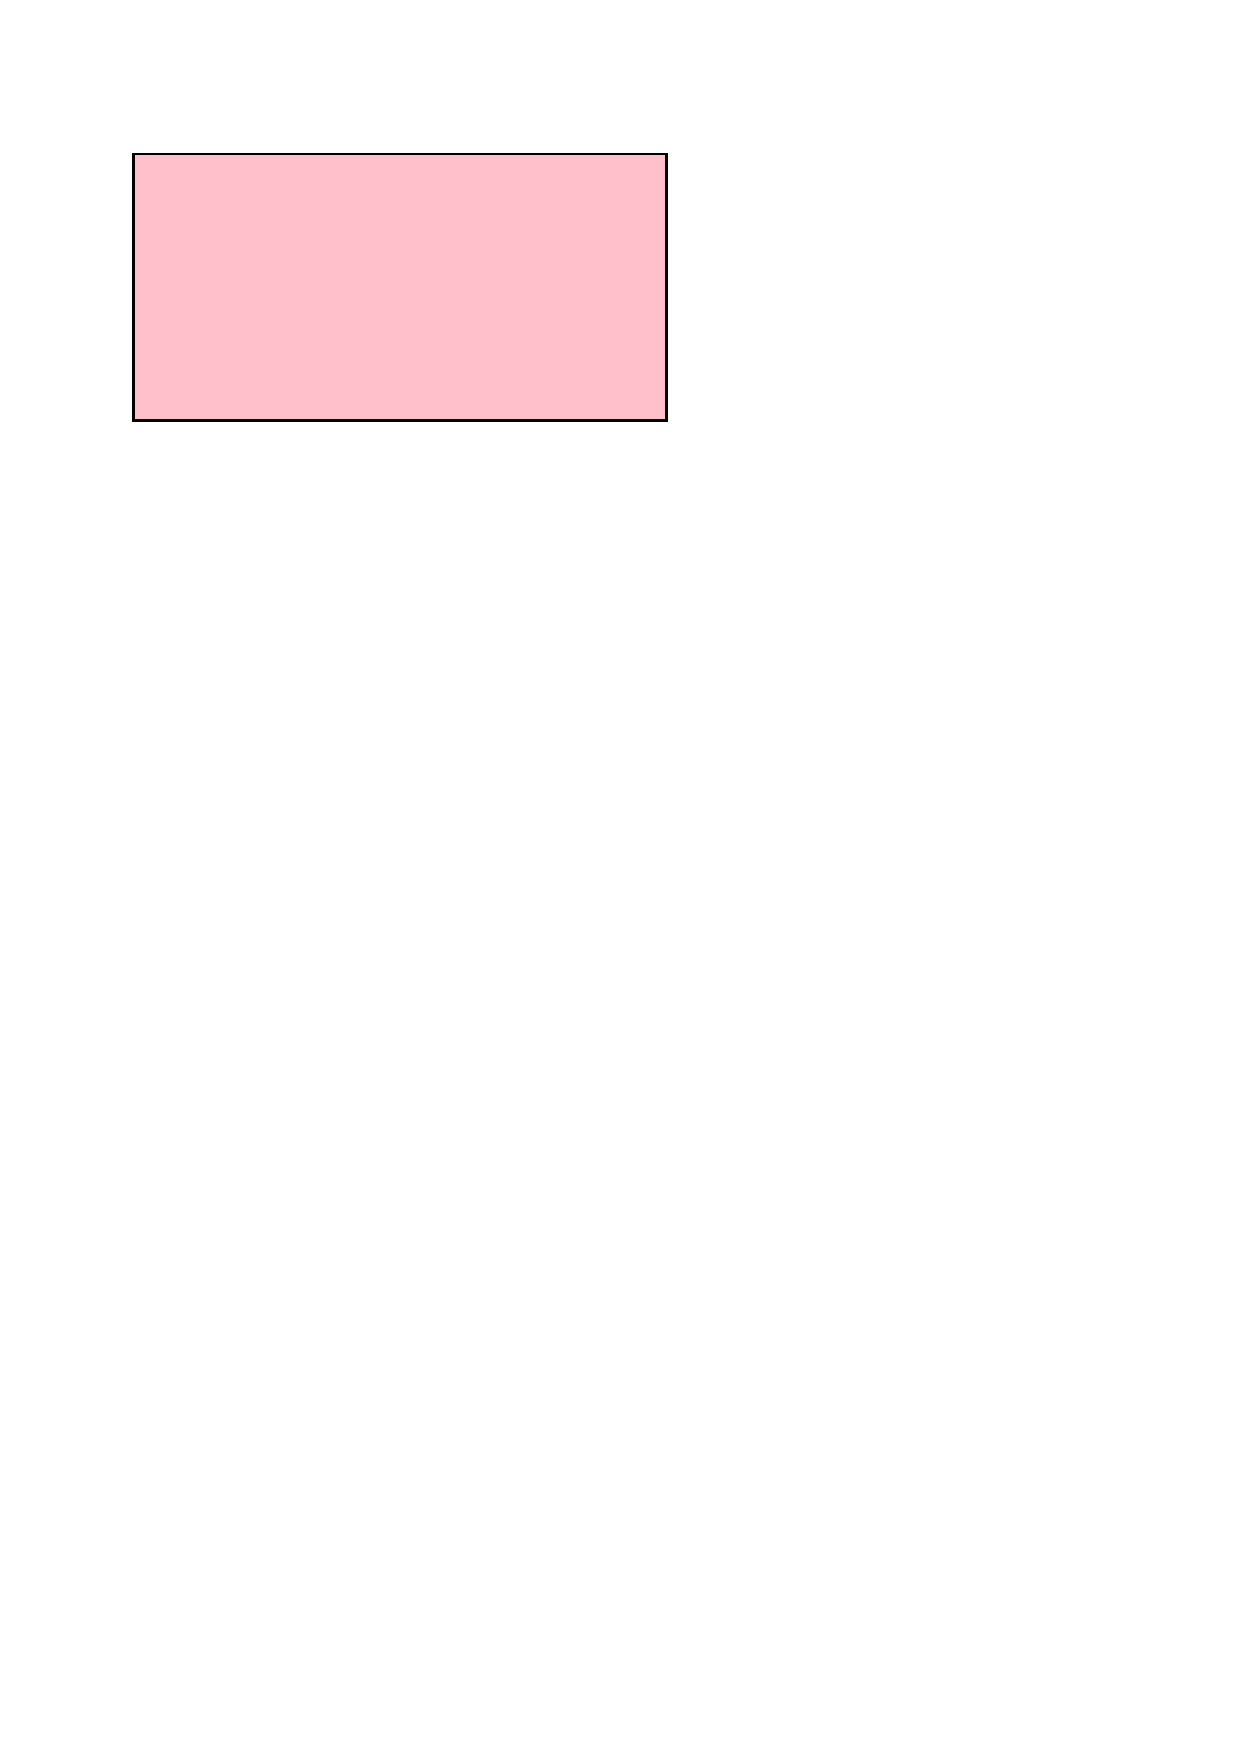
\includegraphics{strides-1}
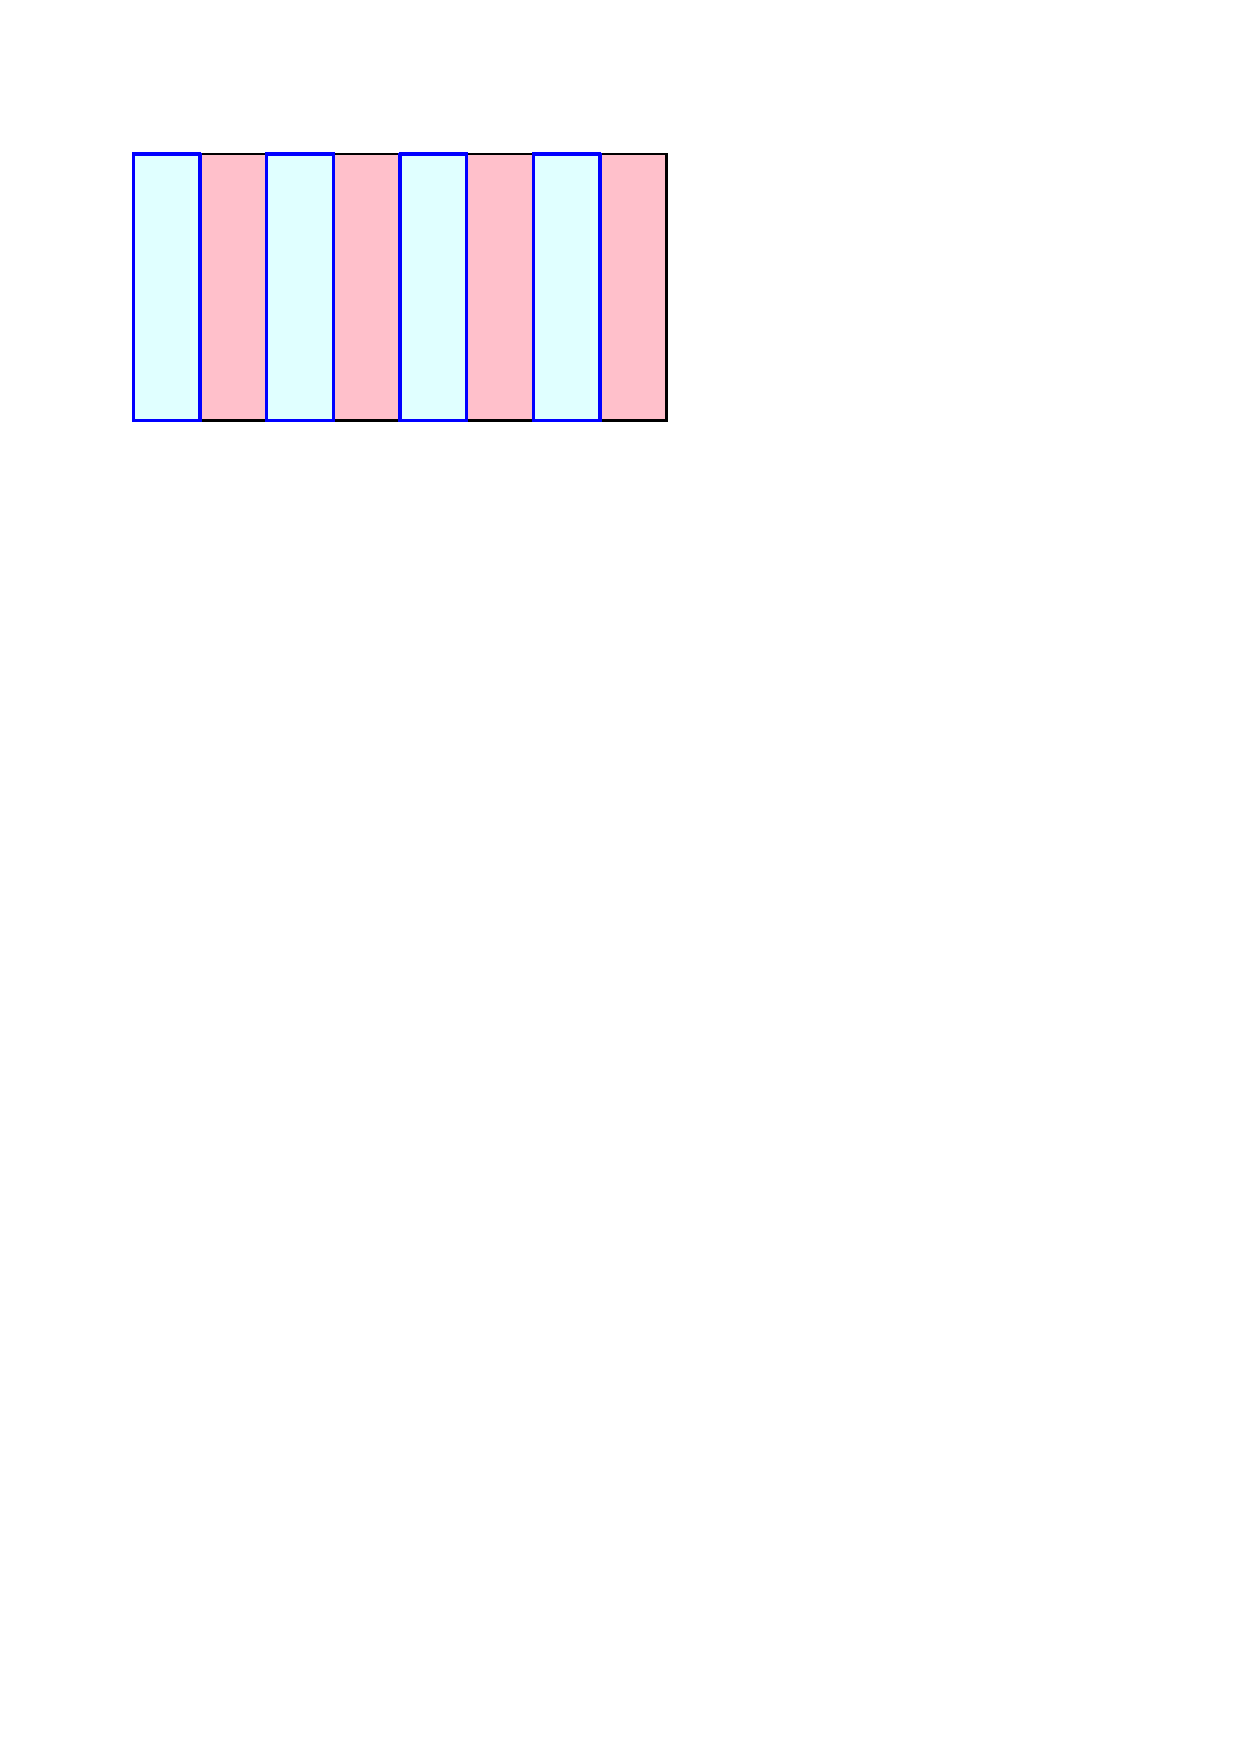
\includegraphics{strides-2}
\end{center}

\vspace{1cm}


\end{minipage}
\hspace{1cm}
}}
\end{textblock}
 
%%%%%%%%%%%%%%%%%%%%%%%%%%%%%%%%%%%%%%%%%%%%%%%%%%%%%%%%%%%%%%%%%%%%%%%%%%%%%%%%%%%%%%%%%%%%%%%%%%
%%% Broadcasting
 
\begin{textblock}{12}(0,7.7)
\Ovalbox{
\hspace{1cm}
\begin{minipage}{35.85cm}
\vspace{0.8cm}
\begin{center}
{\huge Broadcasting}
\end{center}
%\noindent

%\only<1>{We have matrix ${\color{red!50}A}$ (size [8,8]) and we want to add a bias vector ${\color{cyan!50}b}$ (size [8,1]) to it.}
%\only<2>{So we make virtual copies of ${\color{cyan!50}b}$ along the last dimension until it has the same size as ${\color{red!50}A}$.}
\begin{itemize}
\item We have matrix A (size [8,8]) and we want to add a bias vector b (size [8,1]) to it.
\item This doesn't fit the rules for elementwise operations since both objects do not have the same number of elements.
\end{itemize}
\begin{center}
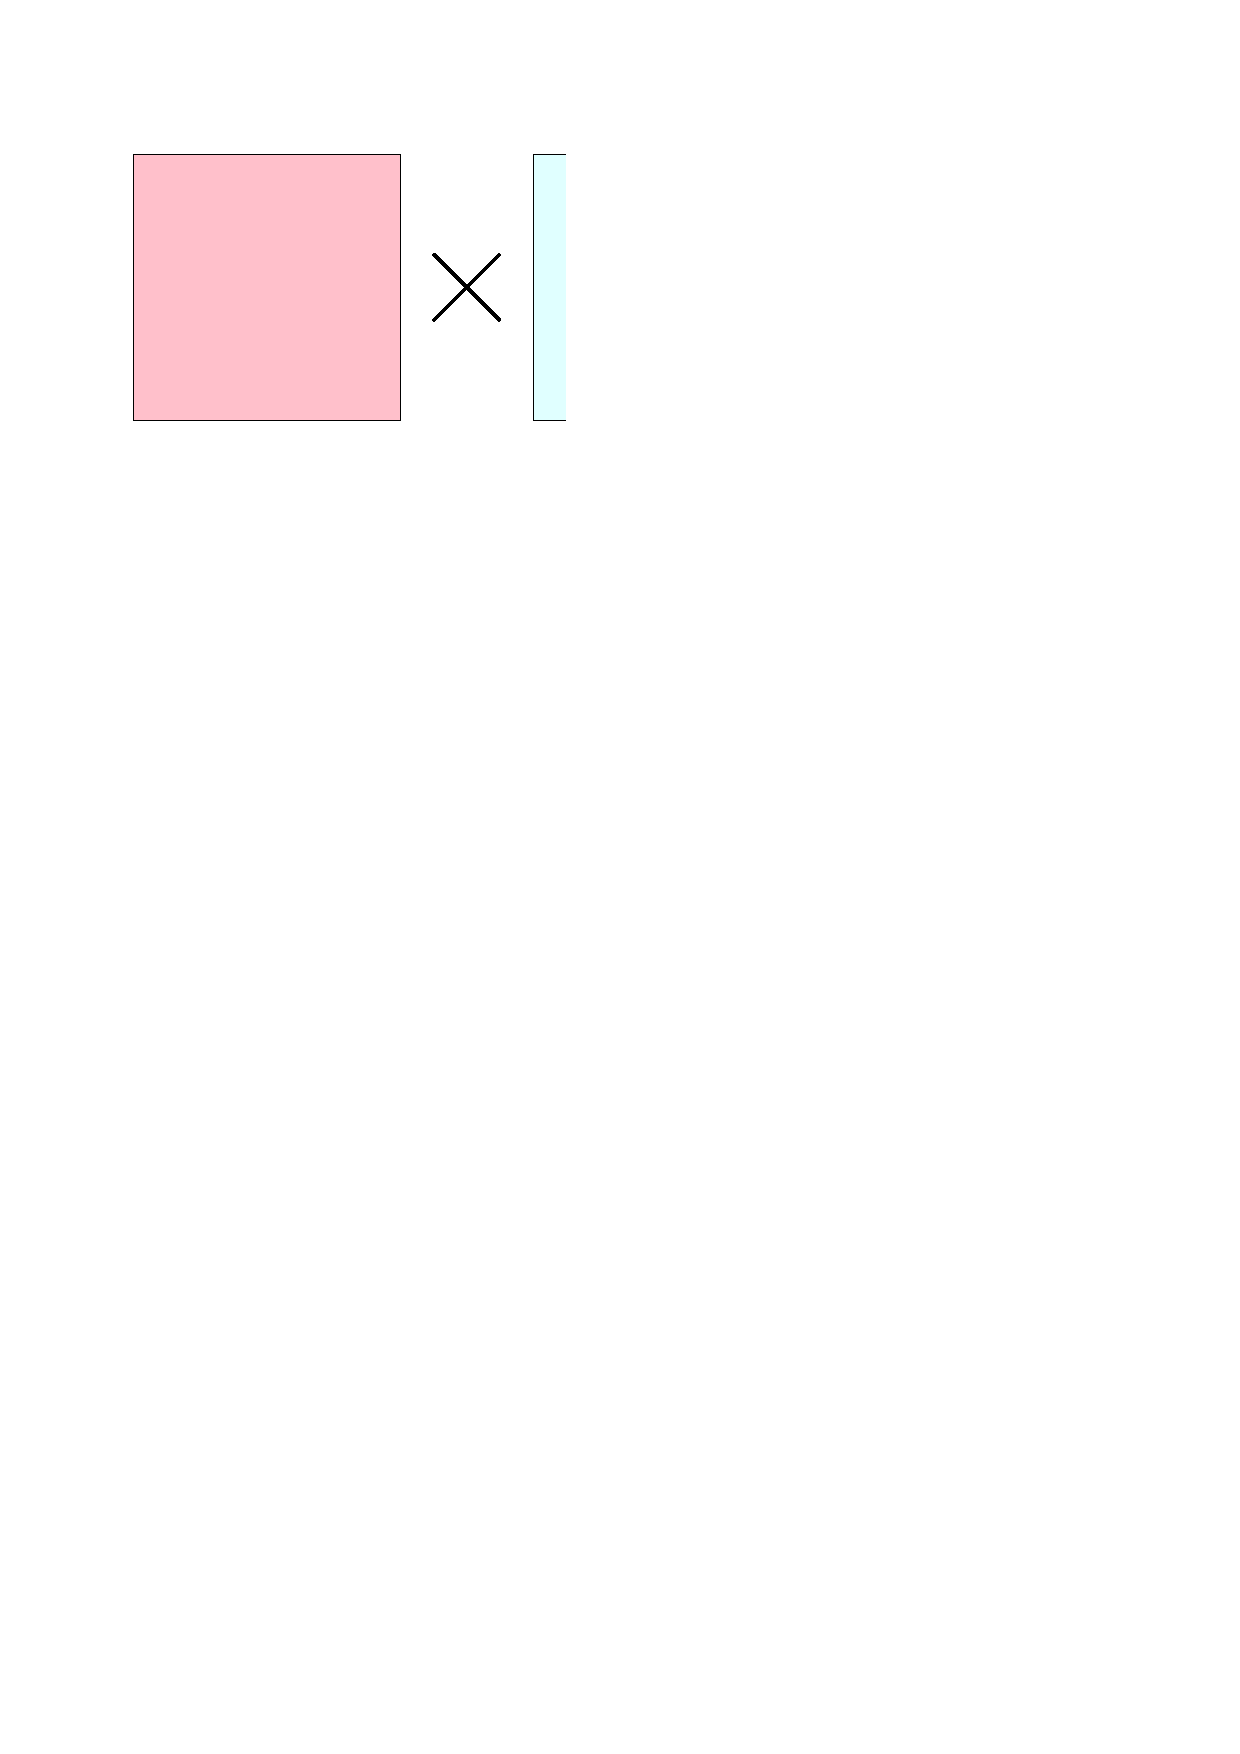
\includegraphics{bcast-1}
\end{center}

\begin{itemize}
\item So we make virtual copies of b along the last dimension until it has the same size as A.
\item Then we can proceed as usual for elementwise.
\end{itemize}

\begin{center}
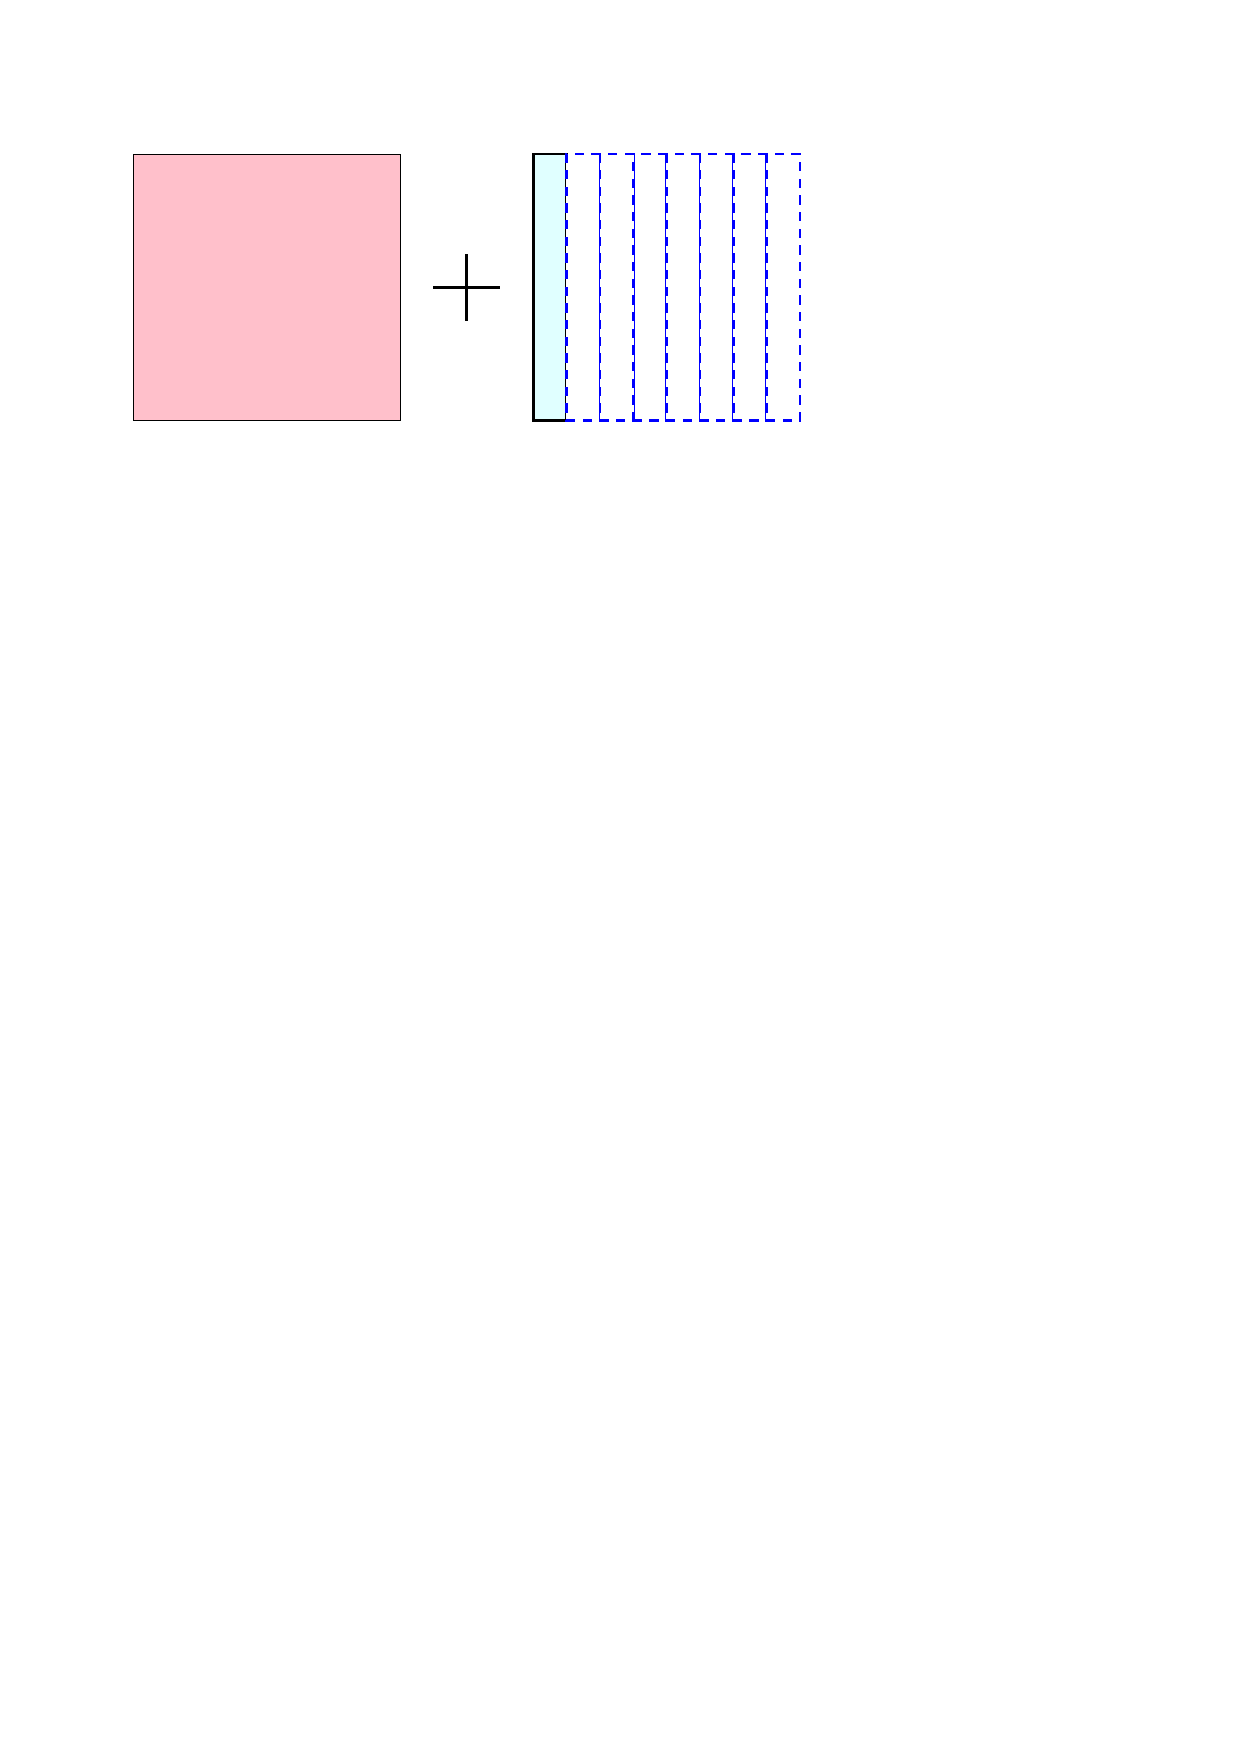
\includegraphics{bcast-2}
\end{center}

\vspace{1cm}
\end{minipage}
\hspace{1cm}
}
\end{textblock}

%%%%%%%%%%%%%%%%%%%%%%%%%%%%%%%%%%%%%%%%%%%%%%%%%%%%%%%%%%%%%%%%%%%%%%%%%%%%%%%%%%%%%%%%%%%%%%%%%%
%%% Operator

 \begin{textblock}{12}(0,10.)

\Ovalbox{

\hspace{1cm}
\begin{minipage}{35.85cm}
\vspace{1cm}
\begin{center}
  {\huge Comparison of existing implementations}
\end{center}

%\begin{table}
%%\rowcolors{2}{RoyalBlue!5}{RoyalBlue!23}
%\begin{tabular}{|l|c|c|c|c|c|}
%\hline
%Package & strides & bcast & dims & types & backends \\
%\hline
%\hline
%Theano & yes\footnote{as number of elements} & yes & any & float32 & CUDA \\
%PyCUDA& no & no & any & all & CUDA \\
%PyOpenCL & no & no & any & all & OpenCL \\
%CUDAMat & no & yes\footnote{via a function} & 2 & float32 & CUDA \\
%Gnumpy & no & yes & any & float32\footnote{and a hackish form of boolean} & CUDA \\
%Thrust & no & no & 1 & all & CUDA \\
%\hline
%%\hiderowcolors
%Desired & yes & yes & any & all & both \\
%\hline
%\end{tabular}
%\end{table}


\vspace{1.13cm}
\end{minipage}
\hspace{1cm}
}
\end{textblock}

 
%%%%%%%%%%%%%%%%%%%%%%%%%%%%%%%%%%%%%%%%%%%%%%%%%%%%%%%%%%%%%%%%%%%%%%%%%%%%%%%%%%%%%%%%%%%%%%%%%%
%%% Nystrom




\begin{textblock}{12}(12,4.9)
\Ovalbox{
\hspace{1cm}
\begin{minipage}{35.85cm}
\vspace{1cm}
   \begin{center}
     {\huge Eigenfunctions}
   \end{center}

   {\large
   
  The previously described algorithms provide a reduced set of coordinates
  only for the training data points: \textbf{the main contribution of our
    work is to show a working extension of these algorithms for computing
    an out-of-sample embedding}.
}

  
{\em  Let $\tilde{K}(a,b)$ be a kernel function, not necessarily positive semi-definite,
with a discrete spectrum,
  that gives rise to a symmetric matrix $\tilde{M}$ with entries
  $\tilde{M}_{ij} = \tilde{K}(x_i,x_j)$ upon a dataset
  $D=\{x_1,\ldots,x_n\}$.  Let $(v_k,\lambda_k)$ be an
  (eigenvector,eigenvalue) pair that solves $\tilde{M} v_k = \lambda_k
  v_k$.  Let $(f_k,\lambda'_k)$ be an (eigenfunction,eigenvalue) pair
  that solves $\tilde{K}_{\hat{p}} f_k = \lambda'_k f_k$ with $\hat{p}$ the empirical distribution
  over $D$. Let $e_k(x)=y_k(x) \sqrt{\lambda_k}$ or $y_k(x)$ denote the embedding associated
with a new point $x$. Then
\begin{eqnarray}
 \lambda'_k &=& \frac{1}{n} \lambda_k \\
\label{eq:eigen-fn}  f_k(x) &=& \frac{\sqrt{n}}{\lambda_k} \sum_{i=1}^n v_{ik} \tilde{K}(x,x_i) \\
 f_k(x_i) &=& \sqrt{n} v_{ik} \\
 y_k(x) &=& \frac{f_k(x)}{\sqrt{n}}=\frac{1}{\lambda_k} \sum_{i=1}^n v_{ik} \tilde{K}(x,x_i) \\
\label{eq:embed}
 y_k(x_i) &=& y_{ik}, \hspace*{6mm} e_k(x_i) = e_{ik}
\end{eqnarray}
If $\tilde{K}(x,y)=\phi(x).\phi(y)$ and $\frac{1}{n}\sum_i\phi(x_i)=0$ then
for $\lambda_k>0$, $e_k(x)$ is the kernel
PCA projection with kernel $\tilde{K}$.
}


{\large
The eigenfunctions define an embedding over the whole space, which is
consistent with the embedding given by the original algorithms on the
training set.  Hence, these formul{\ae} can be used to {\color{Green} estimate an
  embedding for out-of-sample points} without having to reconsider all the
training points.
}

  \vspace{1cm}
\end{minipage}
\hspace{1cm}
}
\end{textblock}


%%%%%%%%%%%%%%%%%%%%%%%%%%%%%%%%%%%%%%%%%%%%%%%%%%%%%%%%%%%%%%%%%%%%%%%%%%%%%%%%%%%%%%%%%%%%%%%%%%
%%% Generalized Kernels

\begin{textblock}{12}(12,1.5)
\Ovalbox{
\hspace{1cm}
\begin{minipage}{35.85cm}
\vspace{1cm}
   \begin{center}
     {\huge Generalized Kernels}
   \end{center}
{\large
  For each algorithm, $\tilde{K}_n$ must be defined over all the sample space.
}
  \begin{itemize}
  \item {\large Spectral Clustering and Laplacian Eigenmaps:}
    \[
 \tilde{K}(a,b) = \frac{1}{n} \frac{K(a,b)}{\sqrt{E_x[K(a,x)]E_{x'}[K(b,x')]}}
\]
\item {\large MDS and Isomap:}
  \[
 \tilde{K}(a,b) = -\frac{1}{2}(d^2(a,b) - E_x[d^2(x,b)]
 - E_{x'}[d^2(a,x')] + E_{x,x'}[d^2(x,x')])
 \]
 {\normalsize
 where $d(a,b)$ is some distance between $a$ and $b$. In the case of
 Isomap, we only use the training points in the intermediates points on the
 path from $a$ to $b$.}
\item {\large LLE:}
\[
 \tilde{K}(a,b) = w(a,b) + w(b,a) - \sum_i w(x_i,a) w(x_i,b).
 \]
 {\normalsize
 with}
 \[
 w(a,b) = 1_{b=x_{n(j)} \in {\cal N}(a)} 
          \frac{\sum_q C^{-1}(x)_{jq}}{\sum_{pq} C^{-1}(x)_{pq}}
          \]
          {\normalsize
and}
\[
C(x)_{ij} = (x - x_{n(i)})(x - x_{n(j)})' 
1_{x_{n(i)} \in {\cal N}(x)}1_{x_{n(j)} \in {\cal N}(x)}
\]
{\normalsize
where ${\cal N}(x)$ is the subset of $k$ elements from $D$
that are the $k$ nearest neighbors of $x$ and $n(i)$ is the
index of the $i$-th such neighbor of $x$.}
  \end{itemize}
  
 
  \vspace{1.35cm}
\end{minipage}
\hspace{1cm}
}
\end{textblock}

%%%%%%%%%%%%%%%%%%%%%%%%%%%%%%%%%%%%%%%%%%%%%%%%%%%%%%%%%%%%%%%%%%%%%%%%%%%%%%%%%%%%%%%%%%%%%%%%%
%%% References 

\begin{textblock}{6}(12,9.47)
\Ovalbox{
\hspace{1cm}
\begin{minipage}{35.85cm}
  \vspace{0.9cm}
\begin{thebibliography}{}
\bibitem[\protect\citename{Belkin and Niyogi}2003]{Belkin+Niyogi-2003}
Belkin, M. and Niyogi, P.\bibleft2003\bibright.
\newblock Laplacian eigenmaps for dimensionality reduction and data
  representation.
  \newblock {\em Neural Computation}, 15(6):1373--1396.

  \bibitem[\protect\citename{Ng, Jordan and Weiss}2002]{Ng2002}
Ng, A.~Y., Jordan, M.~I., and Weiss, Y.\bibleft2002\bibright.
\newblock On spectral clustering: Analysis and an algorithm.
\newblock In Dietterich, T.~G., Becker, S., and Ghahramani, Z., editors, {\em
  Advances in Neural Information Processing Systems 14}, Cambridge, MA. MIT
Press.

\bibitem[\protect\citename{Roweis and Saul}2000]{roweis00lle}
Roweis, S. and Saul, L.\bibleft2000\bibright.
\newblock Nonlinear dimensionality reduction by locally linear embedding.
\newblock {\em Science}, 290(5500):2323--2326.


\bibitem[\protect\citename{Tenenbaum, {de Silva} and
  Langford}2000]{Tenenbaum2000-isomap}
Tenenbaum, J., {de Silva}, V., and Langford, J.\bibleft2000\bibright.
\newblock A global geometric framework for nonlinear dimensionality reduction.
\newblock {\em Science}, 290(5500):2319--2323.

\bibitem[\protect\citename{Williams and Seeger}2000]{Williams+Seeger-2000}
Williams, C. and Seeger, M.\bibleft2000\bibright.
\newblock The effect of the input density distribution on kernel-based
  classifiers.
\newblock In {\em Proceedings of the Seventeenth International Conference on
  Machine Learning}. Morgan Kaufmann.
\end{thebibliography}{}
More references in the paper.

\vspace{0.82cm}
\end{minipage}
\hspace{1cm}
}
\end{textblock}


%\begin{textblock}{10}(0,0)
%\includegraphics{background.eps}
%\end{textblock}


%%%%%%%%%%%%%%%%%%%%%%%%%%%%%%%%%%%%%%%%%%%%%%%%%%%%%%%%%%%%%%%%%%%%%%%%%%%%%%%%%%%%%%%%%%%%%%%%%
%%% Minimization problem

%% \begin{textblock}{6}(14.5,6.7)
%% {\color{Green}
%% \Ovalbox{
%% {\color{Black}
%% \hspace{1cm}
%% \begin{minipage}{30cm}
%% \vspace{1cm}
%% \begin{center}
%% {\huge Minimization Problem}
%% \end{center}
%% \noindent
%% {\Large
%% Asymptotically, the spectral embedding for a kernel $K$ is the solution
%% of a sequential minimization problem, iteratively minimizing
%% the expected value of the loss criterion $L(x_i,x_j)$. More precisely,
%% with $\{(f_k,\lambda_k)\}_{k=1}^{q-1}$ already obtained,
%% one can recursively obtain $(f_q,\lambda_q)$  by minimizing
%%  \[
%%      \int (K(x_i,x_j)-\sum_{k=1}^q \lambda_k f_k(x)f_k(y))^2 p(x)p(y)dx dy
%%  \]
%% where by convention we scale $f_q$ such that $\int f_q(x)^2 p(x)=1$ (any other scaling
%% can be transferred into $\lambda_q$).
%% If the $K_n$ and the $f_{k,n}$ converge uniformly in probability, the Monte-Carlo
%% average of this criterion
%% \[
%%  \frac{1}{n^2}\sum_{i=1}^{n}\sum_{j=1}^n (K_n(x_i,x_j)-\sum_{k=1}^m \lambda_{k,n} f_{k,n}(x_i)f_{k,n}(x_j))^2
%% \]
%% converges in probability to the above asymptotic expectation.}
%% \vspace{1cm}
%% \end{minipage}
%% \hspace{1cm}
%% }}}
%% \end{textblock}
 
\end{document}


